\documentclass{article}

\usepackage[spanish]{babel} % Idioma del CV en español.
\usepackage[utf8]{inputenc} % Para caracteres especiales. 

\usepackage[a4paper]{geometry} % Definimos estilos de página.
\geometry{top=0.5cm, bottom=0cm, left=0.5cm, right=0cm} % Eliminamos todos los márgenes posibles.

%----------------------------------------------------------------------------------------------- 
% TEXTO E ICONOS
%-----------------------------------------------------------------------------------------------

\setlength{\parindent}{0mm} % Determinas la sangría en cero.

\usepackage{fetamont} % Fuente.
\usepackage[T1]{fontenc} % Si no usamos este paquete::
                            % * Las palabras que contienen caracteres acentuados no se pueden separar automáticamente,
                            % * No se puede copiar y pegar correctamente tales palabras de la salida (DVI/PS/PDF),
                            % * Y caracteres como el signo de barra vertical, el signo menor que y el signo mayor dan resultados inesperados en el texto.
\usepackage{moresize} % Más tamaños de fuentes.

\usepackage{ragged2e} % Alineación del texto.
\usepackage{fontawesome} % Set de iconos.
\usepackage{paracol} % Para mostrar dos columnas rompibles.

\usepackage{fancyhdr} % Nos proporciona amplias funciones, tanto para construir encabezados y pies de página, como para controlar su uso (por ejemplo, en momentos en que LATEX cambiaría automáticamente el estilo de encabezado en uso).
\pagestyle{empty} % Este comando produce cabeceras y pies de paginas vacíos - sin números de página.

%----------------------------------------------------------------------------------------------- 
% COLOR Y TRANSPARENCIAS
%-----------------------------------------------------------------------------------------------

\usepackage{transparent} % Cómo se puede usar una pila de colores separada para la transparencia, una propiedad además del color.

\usepackage{xcolor} %Ponemos un poco de color, si usamos solo \usepackage{color} tendremos un problema de compatibilidad con el paquete paracol.

\definecolor{maincol}{RGB}{ 225, 0, 0 }
\definecolor{accentcol}{RGB}{ 250, 150, 10 }
\definecolor{darkcol}{RGB}{ 70, 70, 70 }
\definecolor{white}{RGB}{255,255,255} 
\definecolor{darkgray}{HTML}{333333} 
\definecolor{gray}{HTML}{4D4D4D}
\definecolor{sidecolor}{HTML}{E7E7E7}
\definecolor{lightgray}{HTML}{999999}
\definecolor{green}{HTML}{C2E15F}
\definecolor{orange}{HTML}{FDA333}
\definecolor{purple}{HTML}{D3A4F9}
\definecolor{red}{HTML}{FB0B00}
\definecolor{blue}{HTML}{6CE0F1}
\definecolor{mainblue}{HTML}{0E5484}
\definecolor{cerulean}{HTML}{007BA7}
\definecolor{maingray}{HTML}{B9B9B9}
\definecolor{maindarkgray}{HTML}{B3B3B3}

%----------------------------------------------------------------------------------------------- 
%   VARIOS
%----------------------------------------------------------------------------------------------- 

\usepackage[hidelinks]{hyperref} % Para usar links.

\usepackage{tikz} % Para usar gráficos.
\usetikzlibrary{shapes, backgrounds,mindmap, trees}

\usepackage{graphicx} % Para la imagen de la cabecera.
\usepackage{float} % Para poner imágenes donde queremos. 


%----------------------------------------------------------------------------------------------- 
% COSAS QUE NO SE SI VOY A USAR
%----------------------------------------------------------------------------------------------- 

%----------------------------------------------------------------------------------------------- 
%   TABLA/ARRAY
%----------------------------------------------------------------------------------------------- 

\usepackage{array} % Para tener un mejor manejo de tablas.
\usepackage{multirow}


% \usepackage{xstring, xifthen} % Nos proporcionan una prueba \isempty
% \usepackage[absolute,overlay]{textpos}

%----------------------------------------------------------------------------------------------- 
%   SECCIONES DEL CV
%----------------------------------------------------------------------------------------------- 

\newcommand{\cvsection}[1] {
    \vspace{10pt}
	\textbf{\Large{\textcolor{darkcol}{\uppercase{#1}}}}\\[-4pt]
        \textcolor{maincol}{ \rule{0.1\textwidth}{2pt} } 
    \vspace{8pt}
	}

%----------------------------------------------------------------------------------------------- 
%   HABILIDADES
%----------------------------------------------------------------------------------------------- 

\newcommand{\mpwidth}{\linewidth-\fboxsep-\fboxsep}

% Comando para la barra de progreso de habilidades:
% Renders a progress-bar to indicate a certain skill in percent.
% param 1: name of the skill / tech / etc.
% param 2: percent, values range from 0 to 1
\newcommand{\cvskill}[2] {
    \vspace{0pt}
    \textcolor{black}{\textbf{#1}} 
    \newline	
    \begin{tikzpicture}[scale=1,rounded corners=2pt,very thin]
		\fill [lightgray] (0,0) rectangle (1\mpwidth, 0.15);
		\fill [maincol] (0,0) rectangle (#2\mpwidth, 0.15);
  	\end{tikzpicture} 
    \vspace{2pt}
}

%===============================================================================================%
%   CONTENIDO DEL DOCUMENTO
%===============================================================================================%

\begin{document}

\columnratio{0.3} % Donde comienza la siguiente columna de texto.
\setlength{\columnsep}{2em} % Sangria de la siguiente columna de texto.
\setlength{\columnseprule}{4pt} % Linea vertical entre columnas y su espesor.
\colseprulecolor{maingray} % Color de la linea vertical.

\begin{paracol}{2}

%===============================================================================================%
%   BARRA LATERAL
%===============================================================================================%

\begin{leftcolumn}

    \begin{figure}[t]
        \centering
        \noindent    
        \begin{tikzpicture}[remember picture,overlay]
            \node [rectangle, fill=sidecolor, anchor=north, minimum width=16.5cm, minimum height=\paperheight+1cm] (box) at (-5cm,0.5cm){};
        \end{tikzpicture}    
        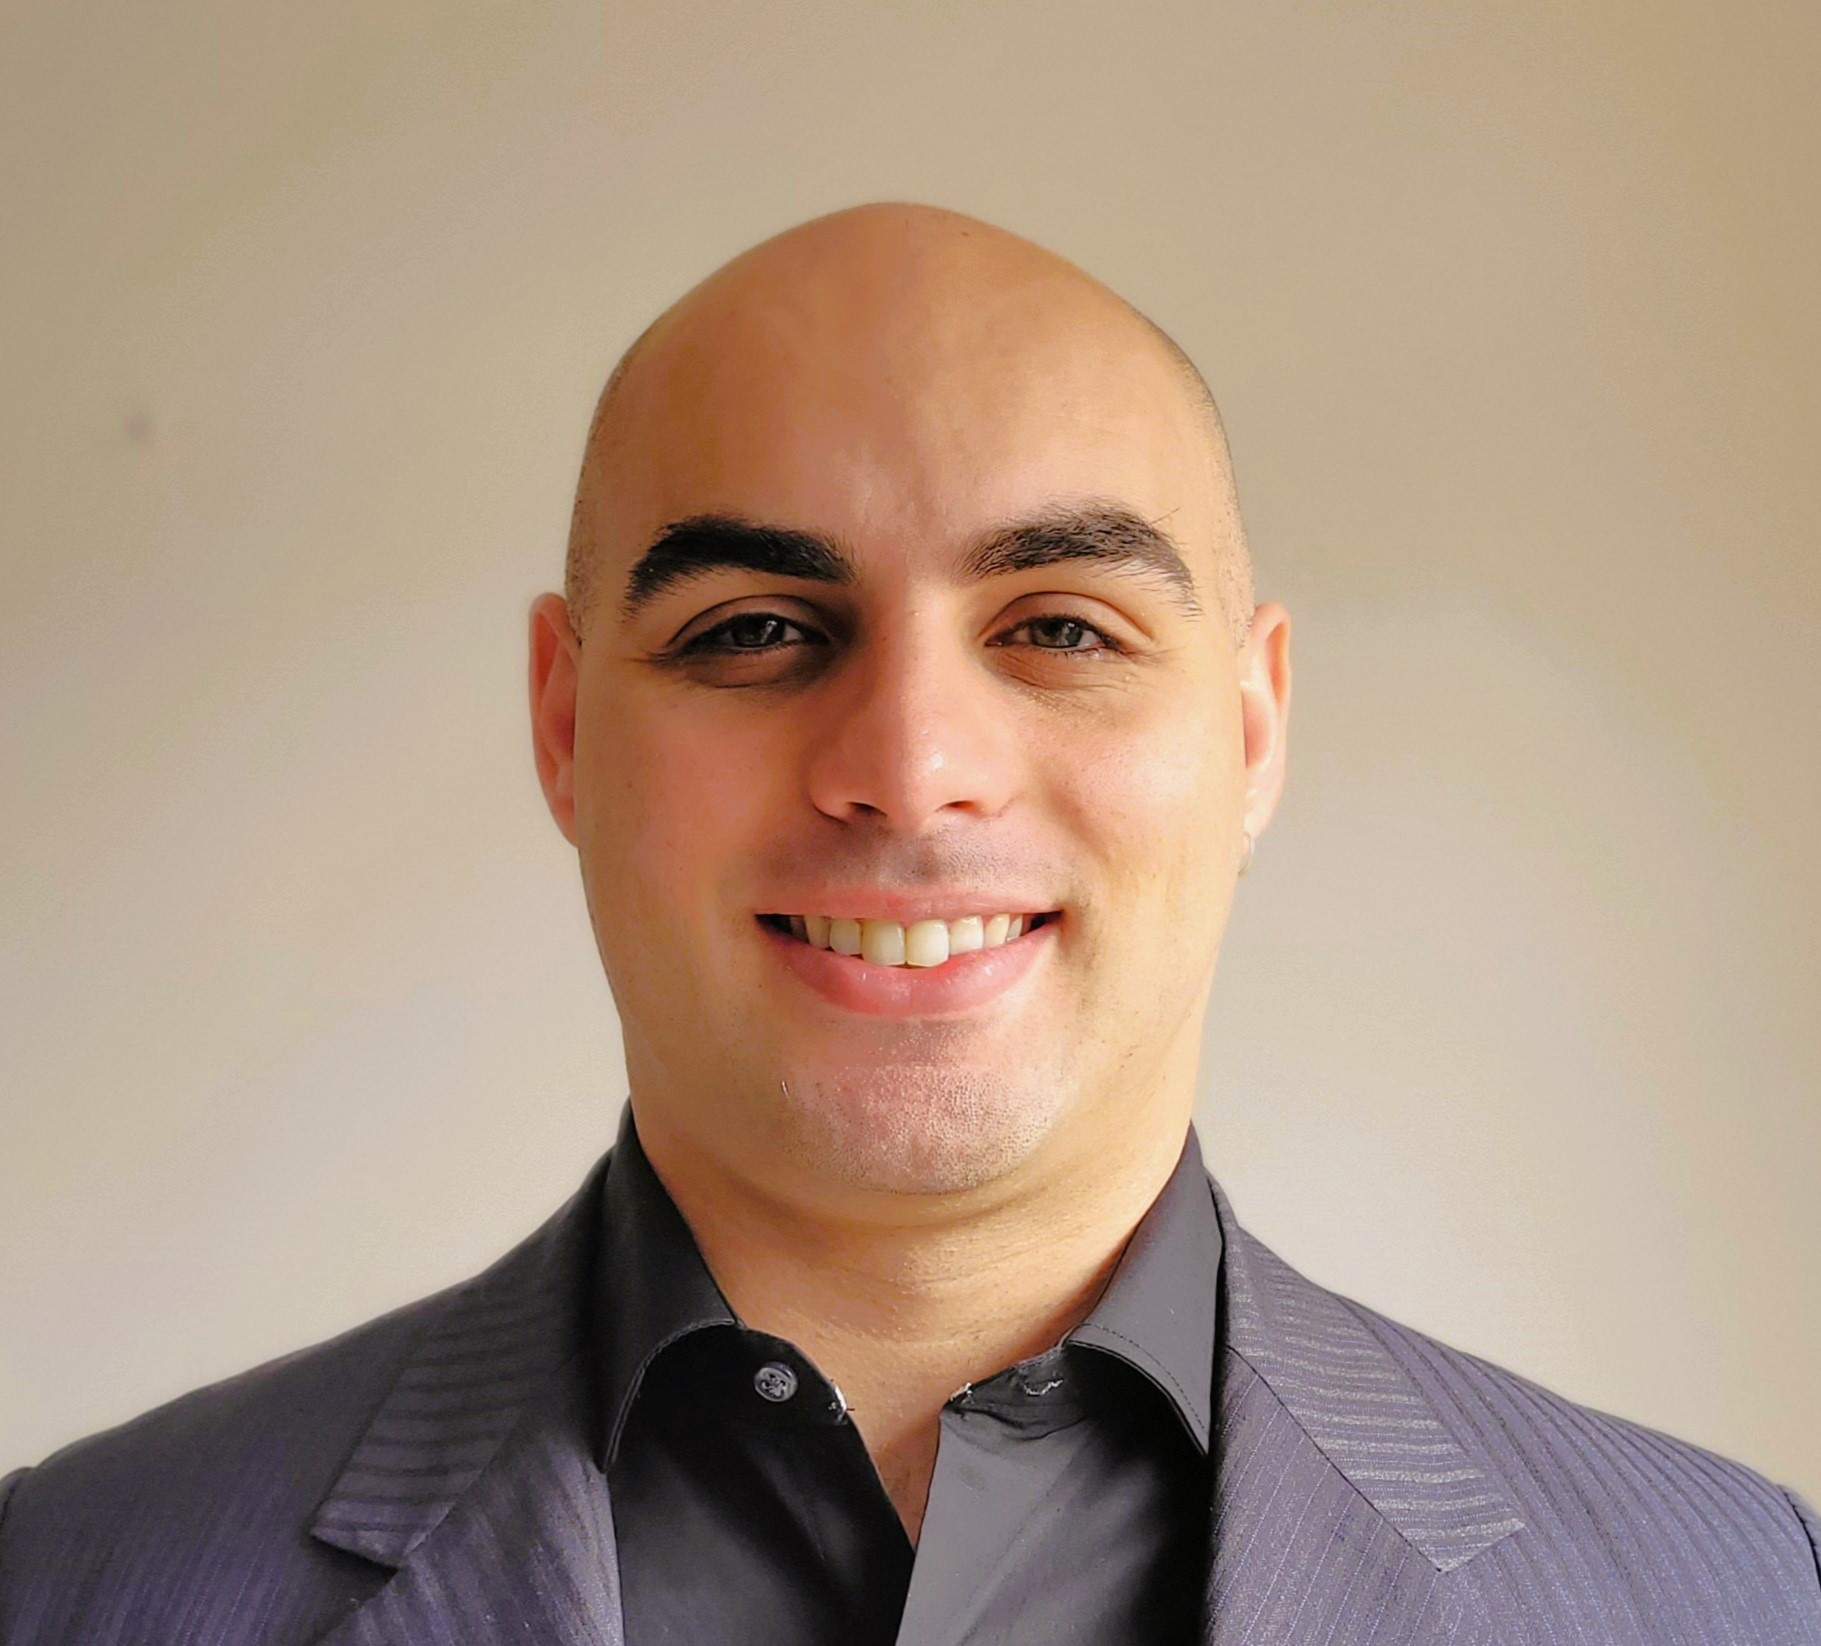
\includegraphics[width=\linewidth]{Foto.jpg}
    \end{figure}
    
    \cvsection{CONTACTO}

    \begin{tabular}{cl}
        {\Large\color{maincol}\faCalendar}                        & 01 de abril de 1992                                                       \\ [2pt]
        \multirow{2}{*}{{\Large\color{maincol}\faInfoCircle}}     & \href{https://goo.gl/maps/ciK9KomkCkJ7PdWt5}{Bahía Blanca} \href{https://goo.gl/maps/hbpY43DfhsFnmc8e6}{Buenos Aires,} \\ [2pt]
                                                                  & \href{https://goo.gl/maps/uPrySfuBds1QBUmq8}{Argentina}                   \\ [2pt]
        {\Large\color{maincol}\faAt}                              & \href{mailto:juanmcarini@gmail.com}{juanmcarini@gmail.com}                \\ [2pt]
        {\Large\color{maincol}\faPhone}                           & \href{tel:+5492914143811}{+54 (0291) 414 3811}                            \\ [2pt]
        {\Large\color{maincol}\faGithub}                          & \href{https://github.com/JuanMCarini}{JuanMCarini}                        \\ [2pt]
        {\Large\color{maincol}\faLinkedinSquare}                  & \href{https://www.linkedin.com/in/juanmcarini}{juanmcarini}
    \end{tabular}

    \cvsection{IDIOMAS}

    \begin{tabular}{ll}
        \textbf{Español:} & nativo \\ [2pt]
        \textbf{Ingles:}  & básico profesional.
    \end{tabular}

    \cvsection{HABILIDADES}

    \cvskill{SQL}      {0.3} 
    \cvskill{Python}   {0.4}
    \cvskill{Power BI} {0.5}
    \cvskill{Excel}    {0.8}
    \cvskill{LaTex}    {0.8}

\end{leftcolumn}

\begin{rightcolumn}
%===============================================================================================%
%   CABECERA
%===============================================================================================%
\fcolorbox{white}{darkcol}{\begin{minipage}[c][5cm][c]{0.96\mpwidth}
	\begin{center}
		\HUGE{ \textbf{ \textcolor{white}{ \uppercase{CARINI \\ JUAN MARTÍN} } } } \\[-12pt]
		\textcolor{white}{ \rule{0.1\textwidth}{1.25pt} } \\[4pt]
		\large{\textcolor{white} {Lic.\@ en Matemática \& Científico de Datos}}
	\end{center}
\end{minipage}}
\vspace{6pt}

\cvsection{EDUCACIÓN}



\end{rightcolumn}

\end{paracol}

\end{document}